%This is a very basic  BE PROJECT PRELIMINARY template.

%############################################# 
%#########Author :  PROJECT###########
%#########COMPUTER ENGINEERING############


\documentclass[oneside,a4paper,12pt]{report}
%\usepackage{showframe}
%\hoffset = 8.9436619718309859154929577464789pt
%\voffset = 13.028169014084507042253521126761pt

\fancypagestyle{plain}{%
  \fancyhf{}
  \fancyfoot[CE]{College_Name, Department of Computer Engineering 2015}
  \fancyfoot[RE]{\thepage}
}
\pagestyle{fancy}
\fancyhead{}
\renewcommand{\headrulewidth}{0pt}
\footskip = 0.625in
\cfoot{}
\rfoot{}

\usepackage[]{hyperref}
\usepackage{tikz}
\usetikzlibrary{arrows,shapes,snakes,automata,backgrounds,petri}

\usepackage{tabularx}

\usepackage[nottoc,notlot,notlof,numbib]{tocbibind}
\usepackage[titletoc]{appendix}
\usepackage{titletoc}

\renewcommand{\appendixname}{Annexure}
\renewcommand{\bibname}{References}

\setcounter{secnumdepth}{5}

\usepackage{float}
\usepackage{subcaption}
\usepackage{multirow}

\usepackage[ruled,vlined]{algorithm2e}

\begin{document}

\setlength{\parindent}{0mm}
\begin{center}

{\bfseries A PRELIMINARY REPORT ON \\}
 \vspace*{2\baselineskip}
{\bfseries \fontsize{16}{12} \selectfont  Soil based Crop Prediction 		 and Whether Forecasting \\ \vspace*{2\baselineskip}}
{\fontsize{12}{12} \selectfont SUBMITTED TO THE SAVITRIBAI PHULE PUNE UNIVERSITY, PUNE\\
IN THE PARTIAL FULFILLMENT OF THE REQUIREMENTS \\
FOR THE AWARD OF THE DEGREE \\
\vspace*{0\baselineskip}
OF
\vspace*{2\baselineskip}}\\
{\bfseries \fontsize{14}{12} \selectfont BACHELOR OF ENGINEERING (COMPUTER ENGINEERING)  \\
\vspace*{1\baselineskip}} 
{\bfseries \fontsize{14}{12} \selectfont BY \\ 
\vspace*{1\baselineskip}} 
Student Name  \hspace{25 mm} Exam No:  \\
Student Name \hspace{25 mm} Exam No:   \\
Student Name \hspace{25 mm} Exam No:  \\
Student Name \hspace{25 mm} Exam No:\\
\vspace*{1\baselineskip}
{\bfseries \fontsize{14}{12} \selectfont Under The Guidance of \\  
\vspace*{0\baselineskip}} 
Prof. Guide Name\\
\includegraphics[width=100pt]{logos.png} \\
{\bfseries \fontsize{14}{12} \selectfont DEPARTMENT OF COMPUTER ENGINEERING
\\

SHRI CHHATRAPATI SHIVAJI MAHARAJ COLLEGE OF ENGINEERING
\\

NEPTI,AHMEDNAGAR
\\
SAVITRIBAI PHULE PUNE UNIVERSITY 
\\
2021-22

}
\end{center}

\newpage



\begin{figure}[ht]
\centering
\includegraphics[width=100pt]{logos.png}
\end{figure}

{\bfseries \fontsize{16}{12} \selectfont \centerline{CERTIFICATE} 
\vspace*{2\baselineskip}} 

\centerline{This is to certify that the project report entitles}
\vspace*{1\baselineskip} 


{\bfseries \fontsize{14}{12} \selectfont \centerline{Soil based Crop Prediction 		 and Whether Forecasting}
\vspace*{1\baselineskip}}

\centerline{Submitted by}
\vspace*{1\baselineskip} 
\centerline{Student Name  \hspace{25 mm} Exam No: } 
\centerline{Student Name \hspace{25 mm} Exam No:  } 
\centerline{Student Name \hspace{25 mm} Exam No: }
\centerline{Student Name \hspace{25 mm} Exam No: }

is a bonafide student of this institute and the work has been carried out by him/her under the supervision of  \textbf{Prof. A. B. C} and it is approved for the partial fulfillment of the requirement of Savitribai Phule Pune University, for the award of the degree of Bachelor of Engineering (Computer Engineering). \\\\

\bgroup
\def\arraystretch{0.7}
\begin{tabular}{c c }
Prof. Guide Name &  \hspace{60 mm} Prof. (......)  \\								
Internal Guide   &  \hspace{60 mm}External Name  \\
Dept. of Computer Engg.  &	\hspace{50 mm}\\

\end{tabular}


%}

\vspace*{2\baselineskip}
\bgroup
\def\arraystretch{0.4}
\begin{tabular}{c c }
(Prof. J.U. Lagad )  &  \hspace{25 mm} (Dr.M.P.Nagarkar )   \\						 Head  &  \hspace{25 mm} Principal \\
Department of Computer Engineering &	\hspace{25 mm}Shri Chhatrapati Shivaji Maharaj COE   \\
\end{tabular}
%}
\vspace*{0\baselineskip}
\item Place :\\
Date :

\newpage

%\pictcertificate{TITLE OF BE PROJECT}{Student Name}{Exam Seat No}{Guide Name}
\setcounter{page}{0}
\frontmatter
\cfoot{College Short Form Name, Department of Computer Engineering 2021}
\rfoot{\thepage}
\pagenumbering{Roman}
%\pictack{BE PROJECT TITLE}{Guide Name}


{  \newpage {\bfseries \fontsize{14}{12} \selectfont \centerline{Acknowledgments} 
\vspace*{2\baselineskip}} \setlength{\parindent}{11mm} }
{ \setlength{\parindent}{0mm} }
Please Write here Acknowledgment.Example given as\\
\textit{It gives us great pleasure in presenting the preliminary project report 
on {\bfseries \fontsize{12}{12} \selectfont `Soil based Crop Prediction and Whether Forecasting'}.}
\vspace*{1.5\baselineskip}

 \textit{I would like to take this opportunity to thank my internal guide
 \textbf{Prof. Guide Name} for giving me all the help and guidance I needed. I am
 really grateful to them for their kind support. Their valuable suggestions were very helpful.} \vspace*{1.5\baselineskip}

 \textit{I am also grateful to \textbf{Prof.(Prof. J.U. Lagad ) }, Head of Computer
 Engineering Department, CollegeName for his indispensable
 support, suggestions.}
\vspace*{1.5\baselineskip}

\textit{In the end our special thanks to \textbf{Other Person Name} for
providing various resources such as  laboratory with all needed software platforms,
continuous Internet connection, for Our Project.}
\vspace*{3\baselineskip} \\
\begin{tabular}{p{8.2cm}c}
&Student Name1\\
&Student Name2\\
&Student Name3\\
&Student Name4\\
&(B.E. Computer Engg.)
%}
\end{tabular}

		
{  \newpage {\bfseries \fontsize{14}{12} \selectfont \centerline{Abstract} 
In general, agriculture is the backbone of India 
and also plays an important role in Indian economy by providing 
a certain percentage of domestic product to ensure the food 
security. But now-a-days, food production and prediction is 
getting depleted due to unnatural climatic changes, which will 
adversely affect the economy of farmers by getting a poor yield 
and also help the farmers to remain less familiar in forecasting the 
future crops. This research work helps the beginner farmer in 
such a way to guide them for sowing the reasonable crops by 
deploying machine learning, one of the advanced technologies in 
crop prediction. Naive Bayes, a supervised learning algorithm 
puts forth in the way to achieve it. The seed data of the crops are 
collected here, with the appropriate parameters like temperature, 
humidity and moisture content, which helps the crops to achieve a 
successful growth. In addition as the software, a mobile 
application for Android is being developed. The users are 
encouraged to enter parameters like temperature and their 
location will be taken automatically in this application in order to 
start the prediction process. \\
\vspace*{2\baselineskip}} \setlength{\parindent}{11mm} }
{ \setlength{\parindent}{0mm} }



% \maketitle
\tableofcontents
\listoffigures 
%\listoftables



\mainmatter


  \titleformat{\chapter}[display]
{\fontsize{16}{15}\filcenter}
{\vspace*{\fill}
 \bfseries\LARGE\MakeUppercase{\chaptertitlename}~\thechapter}
{1pc}
{\bfseries\LARGE\MakeUppercase}
[\thispagestyle{empty}\vspace*{\fill}\newpage]







\setlength{\parindent}{11mm}
\chapter{Introduction}
\section {Introducation}
 There are so many soil series available in India. Every soil series have different features and every soil is suitable for different crop. Sometimes or we can say every time it happens that farmer soil is best for some specific crop but as he don’t know. The main purpose of the proposed work is to create a suitable model for classifying various kinds of soil series data along with suitable crops suggestion.\\ 
Series are recognized by machine learning methods using various chemical features and possible crops for that soil series are suggested using geographical attributes. Soil is one of the key components in agricultural field for yielding crops. Soil classification philosophies follow the existence knowledge and practical circumstances. On the land surfaces of earth, classification of soil creates a link between soil samples and various kinds of natural entity.

 \\

\section{Motivation}
\label{sec:problem}
\item •	Modern technologies have enabled human society to produce enough food to feed more than 7 billion people. However, food security is still jeopardised due to a variety of factors such as climate change, pollinator decline, crop plant diseases, and others. Crop Plant diseases not only pose a global threat to food security, but they can also have disastrous consequences for smallholder farmers whose livelihoods rely on healthy crops. Furthermore, the majority of hungry people (50 percent) live in smallholder farming households, making smallholder farmers particularly vulnerable to pathogen-related disruptions in food supply.\\
\section{Problem Statement}
\label{sec:problem}

\item Crop  prediction is one of the challenging problems in precision agriculture, and many models have been proposed and validated so far.
 This problem requires the use of several datasets since crop yield depends on many different factors such as climate, weather, and soil, use of fertilizer etc. To develop Soil detection and Crop predication system.




\chapter{Literature Survey}
\section {Study Of Research Paper}
\item \textbf{1.Paper Name:} Crop Yield Analysis Using Machine Learning 
Algorithms
\\
\textbf{Author:}Fatin Farhan Haque, Ahmed Abdelgawad, Venkata Prasanth Yanambaka, Kumar Yelamarthi \\
\textbf{Abstract :}:- Agriculture is not only a huge aspect of the 
growing economy, but it’s essential for us to survive. Predicting 
crop yield is not an easy task, as it depends on many parameters 
such as water, ultra-violet (UV), pesticides, fertilizer, and the 
area of the land covered for that region. In this paper, two 
different Machine Learning (ML) algorithms are proposed to 
analyze the crops’ yield. These two algorithms, Support Vector 
Regression (SVR) and Linear Regression (LR), are quite 
suitable for validating the variable parameters in the predicting 
the continuous variable estimation with 140 data points that 
were acquired. The parameters mentioned above are key factors 
affecting the yield of crops. The error rate was measured with 
the help of Mean Square Error (MSE) and Coefficient of 
Determination (R2), where MSE gave out approximately 0.005 
and R2 gave around 0.85. The same dataset has been used for 
quick comparison between the algorithms’ performances. \\

\newpage

\item \textbf{ 2.Paper Name:} :- An Analytical Approach for Soil and Land 
Classification System using Image Processing \\
\textbf{Author:}Prof. A. V. Deorankar\\
\textbf{Abstract :}  — In the last few decades researchers are interested 
in land mapping and its classification due to various reasons. The 
reasons for an increase in the focus of the research community 
are, the increasing demand for agricultural land and soil health 
analysis, as the health of the soil, is essential for the healthy 
production of crops. Image classification is one such approach for
soil and land health analysis. It is a complex process having the 
effects of various factors. This paper has proposed the study of 
current researches, the problems it addressed, and its prospects. 
The emphasis is focused on the analytical study of various 
advanced and efficient classification mechanisms and techniques. 
Here, it has been attempted to study the factors these approaches 
have addressed to improve the accuracy of the classification. 
Proper utilization of the number of features of remotely sensed 
data and selecting the best suitable classifier are most important 
for improving the accuracy of the classification. The knowledgebased classification or Non-parametric classifiers like decision 
tree classifier or neural network have gained more popularity for 
multisource data classification in recent times. However, there is 
still the scope of further research, to reduce uncertainties in the 
improvement of accuracy of the Image classification mechanisms  \\ 
	
\newpage
	
\item \textbf{3.Paper Name:}Crop Yield Prediction using Machine Learning 
Techniques   \\
\textbf{Author name:} Ramesh Medar  \\
\textbf{abstract :} Agriculture is the field which plays an important 
role in improving our countries economy. Agriculture is the 
one which gave birth to civilization. India is an agrarian 
country and its economy largely based upon crop productivity. 
Hence we can say that agriculture can be backbone of all 
business in our country. Selecting of every crop is very 
important in the agriculture planning. The selection of crops 
will depend upon the different parameters such as market 
price, production rate and the different government policies. 
Many changes are required in the agriculture field to improve 
changes in our Indian economy. We can improve agriculture 
by using machine learning techniques which are applied easily 
on farming sector. Along with all advances in the machines and 
technologies used in farming, useful and accurate information 
about different matters also plays a significant role in it. The 
concept of this paper is to implement the crop selection method 
so that this method helps in solving many agriculture and 
farmers problems. This improves our Indian economy by 
maximizing the yield rate of crop production.  \\
\newpage

\item \textbf{4.Paper Name:}A Study on Various Data Mining Techniques for 
Crop Yield Prediction \\
\textbf{Author:}:- Yogesh Gandge \\
\textbf{abstract :}India is a country where agriculture and agriculture 
related industries are the major source of living for the people. 
Agriculture is a major source of economy of the country. It is also 
one of the country which suffer from major natural calamities like 
drought or flood which damages the crop. This leads to huge 
financial loss for the farmers thus leading to the suicide. Predicting 
the crop yield well in advance prior to its harvest can help the 
farmers and Government organizations to make appropriate 
planning like storing, selling, fixing minimum support price, 
importing/exporting etc. Predicting a crop well in advance requires 
a systematic study of huge data coming from various variables like 
soil quality ,pH ,EC,N,P,K etc. As Prediction of crop deals with 
large set of database thus making this prediction system a perfect 
candidate for application of data mining. Through data mining we 
extract the knowledge from the huge size of data. This paper 
presents the study about the various data mining techniques used 
for predicting the crop yield. The success of any crop yield 
prediction system heavily relies on how accurately the features have 
been extracted and how appropriately classifiers have been 
employed. This paper summarizes the results obtained by various 
algorithms which are being used by various authors for crop yield 
prediction, with their accuracy and recommendation.\\

\newpage

\item \textbf{5.Paper Name:}CROP PREDICTION USING PREDICTIVE 
ANALYTICS\\
\textbf{Author:}P. S. Vijayabaskar, Sreemathi.R, Keertanaa.E \\
\textbf{Abstract:}— This work is to construct a model for testing the 
soil fertility. It also suggests the crop which has to be planted 
depending upon the value obtained from the sensor. It also 
provides the regional wise information about the crop in the form 
of graph. We have farmer chat where the farmers can share and 
get idea from the expert by registering in this application. It also 
suggests the fertilizer which has to be added to the soil in order to 
increase the crop productivity. It helps the farmer to analyze the 
fertility of their yard and plant the better crop to increase their 
productivity and profit. It also provides the information about 
the fertilizer to be added in the soil and also provide the 
information about the nearby fertilizer shop.  \\

\newpage

\item \textbf{6.paper Name:}Real-Time Monitoring of Agricultural Land with Crop 
Prediction and Animal Intrusion Prevention using 
Internet of Things and Machine Learning at Edge\\
\textbf{Author:}Nikhil R \\
\textbf{Abstract:}Agriculture is considered as a foundation of life, 
since it is the primary source of food and other raw materials. 
It plays a crucial part in the country's economic development. 
Sadly, many of our farmers cultivate their land using the 
conventional methods. we should replace these obsolete 
techniques of farming with advanced techniques. The 
proposed system describes how the use of the IOT and ML 
techniques can be combined to make the irrigation smart. 
The proposed system saves time avoiding problems like 
constant vigilance over the field by using IOT devices, crop 
prediction helps the farmers to grow suitable crops 
depending on the soil parameters by the use of machine 
learning techniques and it also helps in prevention of the 
intruders like wild animals into the field. It also helps in water 
conservation by supplying the plants / field with minimal 
amount of water automatically through the help of sensors 
depending on the water requirements. and finally, SMS and 
Email notifications will be sent to the farmer mobile phone 
during the abnormal conditions of his farm. The proposed 
system can be used for taking edge decisions in real time. \\

\newpage
\item \textbf{7. Paper Name:}Supervised Classification of Spectral Signatures
from Agricultural Land-Cover in Panama Using the
Spectral Angle Mapper Algorithm\\
\textbf{Author name:}Javier E. Sanchez-Gal ´ an
\textbf{Abstract:}In this article the development of a database of
referenced spectral signatures from agricultural land-cover for
the Republic of Panama is presented. This database consists of
reflectance spectra measured on crops and low vegetation, such
as: rice, chili, onion, watermelon, maize and bare soil and of
satellite images of their plots. Details of the integration process
of the database and software developed for the manipulation of
spectral signatures, are described. The Spectral Angle Mapping
algorithm (SAM) is used for the supervised classification of the
agricultural coverages in the database. On the one hand, results
indicate the possibility of using this classification technique for the
automatic determination of crops and even different phenological
stages in a crop via a satellite image. On the other hand, results
highlight the limitations of using this technique on recently
planted crops and soil flooded by rain or with soil cultivated
with a low agricultural cover crop. We foresee the use of this
methodology and database for agricultural land surveys, crop
management or used in the general organization of the territory\\
\newpage
\item \textbf{8.Paper Name:}Soil Classification and Crop Suggestion using
Image Processing\\
\textbf{Author:}T. Abimala, S. Flora Sashya and K. Sripriya\\
\textbf{Abstract:}- This paper is intended to support agriculture by 
classifying 7 different types of soils like Clay, Clayey Peat, 
Clayey Sand, Humus Clay, Peat, Sandy Clay and Silty Sand, 
and in suggesting suitable crops that could be grown in those 
particular soils using image processing. Pre-processing is done 
by using Low Pass filter. HSV, GLCM, Gabor Wavelet 
algorithms are used for feature extraction. HSV, GLCM are 
used to perform colour based feature extraction. Gabor filters 
are used to perform texture based feature extraction. The 
features obtained from the test image are then compared with 
the features obtained from the images in the dataset. Matching 
of image features is achieved by training the Decision Tree 
classifier with statistical measurements like mean, standard 
deviation, skew and kurtosis. Finally the soil is predicted with 
the help of segmented images that are given as input for 
simulation using Matlab R2018a and is followed by crop 
suggestion. 
\\
\newpage
\item \textbf{9.Paper name:}Supervised Machine learning Approach for 
Crop Yield Prediction in Agriculture Sector\\
\textbf{Author:} Dr. Y. Jeevan Nagendra Kumar1\\
\textbf{Abstract:}—Machine learning (ML) is a crucial perspective 
for acquiring real-world and operative solution for crop 
yield issue. From a given set of predictors, ML can 
predict a target/outcome by using Supervised Learning. 
To get the desired outputs need to generate a suitable 
function by set of some variables which will map the 
input variable to the aim output. Crop yield prediction 
incorporates forecasting the yield of the crop from past 
historical data which includes factors such as 
temperature, humidity, ph, rainfall, crop name. It gives 
us an idea for the finest predicted crop which will be 
cultivate in the field weather conditions. These 
predictions can be done by a machine learning 
algorithm called Random Forest. It will attain the crop 
prediction with best accurate value. The algorithm 
random forest is used to give the best crop yield model 
by considering least number of models. It is very useful 
to predict the yield of the crop in agriculture sector\\


\chapter{Software Requirements Specification}
\section{Introduction}
\subsection{Project Scope}
\item Crop yields and crop yield forecasts directly affect the annual national and international economy and play a major role in the food economy. Crop yields are highly
dependent on irrigation and climate data. More irrigation does not necessarily increase
yield, and therefore, optimization of irrigation and more efficient irrigation systems
are critical. Predicting yield based on different types of irrigation is one way to optimize
the process.
\subsection{User Classes and Characteristics}
User Can Login/registration our system then predict soil series and suggest crops and also detect weather.
\subsection{Assumptions and Dependencies}
\item Assumptions : We have used Python Technique.Input as Soil Image Dataset and Weather. 
\item Dependencies : We have used python libraries like Tensorflow, keras, opencv and Tkinter. Output to detect Soil Type and Suggest Crop and Also predict Weather .
\section{Functional Requirements}
\subsection{Functional Specification:}
\item - The application is user friendly.
\item - It provides an easy interface to user.
\ite - The accessibility or response time of the application should be fast.
 
\subsection{Dependency and Constraints:}
\item - End User application will be developed in Windows OS.
\item - All scripts shall be written in Python
\item - Application design pattern shall be Singleton.

\section {EXTERNAL INTERFACE REQUIREMENT}
\subsection {User Interface}
 \item Application Based on  Soil based crop prediction 		 and whether forecasting. 
 
 \subsection {Hardware Interfaces:}
 \item RAM : 8 GB\\
As we are using Machine Learning Algorithm and Various High Level Libraries Laptop\\
RAM minimum required is 8 GB.\\
Hard Disk : 40 GB\\
Data Set of CT Scan images is to be used hence minimum 40 GB Hard Disk memory is required.\\
Processor : Intel i5 Processor\\


 \subsection {Software Interfaces}
\item  Operating System: Windows 10 (64 Bit)\\
\item IDE: Spyder\\
\item Programming Language : Python\\

\section {NON FUNCTIONAL REQUIREMENT}
\subsection {PerformanceRequirements}
\item The performance of the functions and every module must be well. The overallperformance of the software will enable the users to work eciently.  Perfor-mance  of  encryption  of  data  should  be  fast.   Performance  of  the  providingvirtual environment should be fastSafety Requirement•The application is designed in modules where errors can be detected and xedeasily. This makes it easier to install and update new functionality if required.\\
 \subsection {Safety Requirement}
 \item The application is designed in modules where errors can be detected and fixed easily. This makes it easier to install and update new functionality if required.\\
 
\subsection {Software Quality Attributes}
\item  Our software has many quality attribute that are given below:-\\
\item Adaptability: This software is adaptable by all users.\\
\item Availability: This software is freely available to all users. The availability of the software is easy for everyone.\\
\item Maintainability: After the deployment of the project if any error occurs then it can be easily maintained by the software developer.\\
\item Reliability: The performance of the software is better which will increase the reliabilityof the Software.\\
\item User Friendliness: Since, the software is a GUI application; the output generated is much user friendly in its behavior.\\
\item Integrity: Integrity refers to the extent to which access to software or data by unauthorized persons can be controlled.\\
\item Security: Users are authenticated using many security phases so reliable security is provided.\\
\item Testability: The software will be tested considering all the aspects.\\

\section {SYSTEM REQUIREMENT}
\begin{itemize}
  \subsection{Database Requirements :}
  \item Database : DBSqlite

 \subsection {Hardware Requirements:}
 \item Hardware : intel core\\
 \item Speed : 2.80 GHz\\
 \item RAM : 8GB\\
 \item HardDisk : 500 GB\\
 \item  Key Board: Standard Windows Keyboard
 
 \subsection {Software Requirements :}
\item  Operating System: Windows 10(64 Bit)\\
\item IDE: Spyder\\
\item Programming Language : python version 3.7,3.8\\
\item Libraries: Tensor Flow, OpenCv, Keras,Numpy\\


\end{itemize}


\section{Analysis Models: SDLC Model to be applied}
\item SDLC Models stands for Software Development Life Cycle Models. In this article,
we explore the most widely used SDLC methodologies such as Agile . Each software development life cycle model starts with the analysis, in which the Also, here
are defined the technologies used in the project, team load. One of the basic notions
of the software development process is SDLC models which stands for Software Development Life Cycle models. SDLC – is a continuous process, which starts from
the moment, when it’s made a decision to launch the project, and it ends at the moment of its full remove from the exploitation. There is no one single SDLC model.
They are divided into main groups, each with its features and weaknesses.
 \begin{center}
	\begin{figure}[!htbp]
		\centering
		\fbox{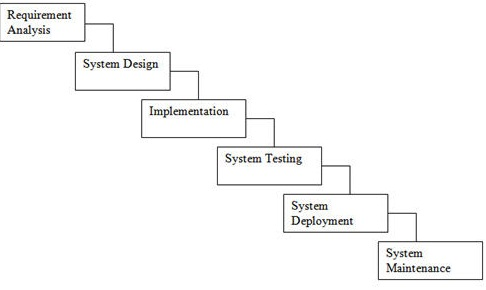
\includegraphics[width=410pt,height=350pt]{Waterfall1.png}}
	  \caption{Waterfall Model}
	  \label{fig:class-dig}
	\end{figure}
\end{center}
\item\textbf{1. Requirement Analysis -} Requirement Analysis is the most important and
necessary stage in SDLC. The senior members of the team perform it with inputs
from all the stakeholders and domain experts or SMEs in the industry. Planning for
the quality assurance requirements and identifications of the risks associated with
the projects is also done at this stage. Business analyst and Project organizer set up
a meeting with the client to gather all the data like what the customer wants to build,
who will be the end user, what is the objective of the product. Before creating a
product, a core understanding or knowledge of the product is very necessary.
\item\textbf{2. System Design -} The next phase is about to bring down all the knowledge
of requirements, analysis, and design of the software project. This phase is the product of the last two, like inputs from the customer and requirement gathering.
\item\textbf{3. Implementation -} In this phase of SDLC, the actual development begins,
and the programming is built. The implementation of design begins concerning writing code. Developers have to follow the coding guidelines described by their management and programming tools like compilers, interpreters, debuggers, etc. are
used to develop and implement the code.
\item\textbf{4. Testing - }After the code is generated, it is tested against the requirements
to make sure that the products are solving the needs addressed and gathered during
the requirements stage. During this stage, unit testing, integration testing, system
testing, acceptance testing are done.
\item\textbf{5. Deployment - }Once the software is certified, and no bugs or errors are
stated, then it is deployed. Then based on the assessment, the software may be
released as it is or with suggested enhancement in the object segment. After the software is deployed, then its maintenance begins.
\item\textbf{6. Maintenance -} Once when the client starts using the developed systems,
then the real issues come up and requirements to be solved from time to time. This
procedure where the care is taken for the developed product is known as maintenance.

\section{System Implementation Plan}

The System Implementation plan table, shows the overall schedule of tasks compilation and
time duration required for each task.

\begin{center}

\begin{tabular}{|c|p{6cm}|p{3cm}|p{3cm}|}
\hline
\textbf{Sr. No.} & \textbf{Name/Title} & \textbf{Start Date}& \textbf{End Date} \\

\hline
1& Preliminary Survey& &  \\
\hline
2& Introduction and Problem Statement
&  &  \\
\hline
3& Literature Survey&      &   \\
\hline
4& Project Statement
&  & \\
\hline
5& Software Requirement And Specification &    & \\
\hline
6 & System Design &  & \\
\hline
7 & Partial Report Submission &  &     \\
\hline
8 & Architecture Design &      &    \\
\hline
9 & Implementation
 &    & \\
\hline
10 & Deployement &      &   \\
\hline
11 & Testing &  &  \\
\hline
12 & Paper Publish
 &  & \\
\hline
13 & Report Submission
 &  &  \\
\hline

\end{tabular}  
%\caption{Schedule of the Project 1}
\end{center}


\newpage
\chapter {System Design}
\section {system Architecture}

\begin{figure}[h]
	\centering
		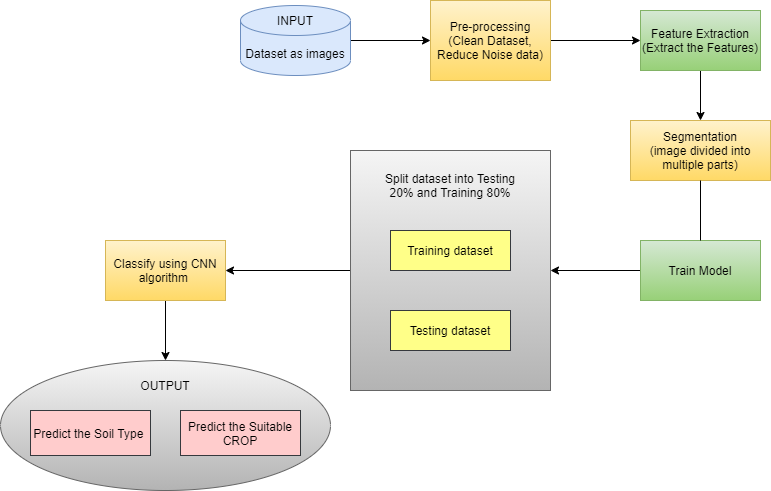
\includegraphics[width=0.90\textwidth]{Crop-Syst-Archi.png}
	\caption {system Architecturel}
	\end{figure}\\



\subsection {Data Flow Diagram}
%\subsection{Data Flow Diagram}  
\item In Data Flow Diagram,we Show that flow of data in our system in DFD0 we show that base DFD in which rectangle present input as well as output and circle show our system,In DFD1 we show actual input and actual output of system input of our system is text or image and output is rumor detected like wise in DFD 2 we present operation of user as well as admin.\\
\begin{center}
	\begin{figure}[!htbp]
		\centering
		\fbox{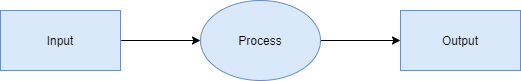
\includegraphics[height=50pt]{DFD-C-0.png}}
	  \caption{Data Flow(0) diagram}
	  \label{fig:act-dig}
	\end{figure}
\end{center}  
\newpage 
\begin{center}
	\begin{figure}[!htbp]
		\centering
		\fbox{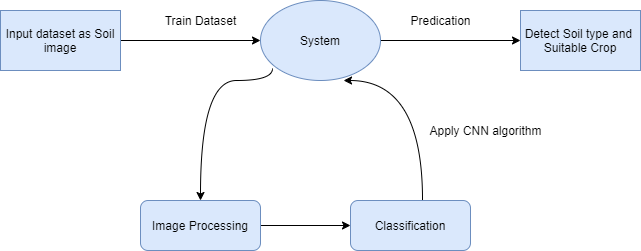
\includegraphics[height=150pt]{DFD-C-1.png}}
	  \caption{Data Flow(1) diagram}
	  \label{fig:act-dig}
	\end{figure}
\end{center}  

\begin{center}
	\begin{figure}[!htbp]
		\centering
		\fbox{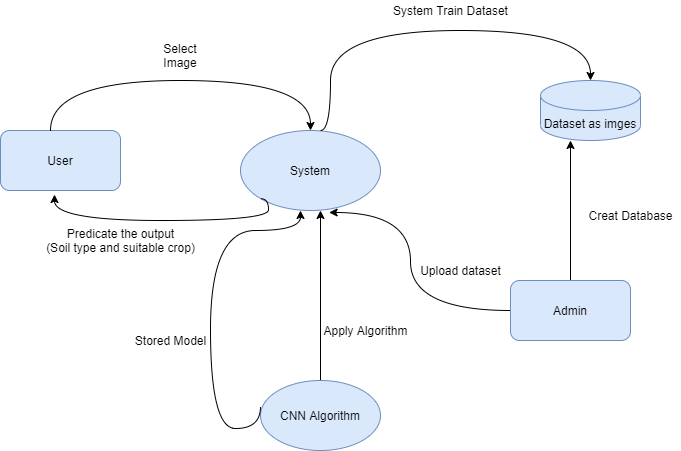
\includegraphics[height=250pt]{DFD-C-2.png}}
	  \caption{Data Flow(2) diagram}
	  \label{fig:act-dig}
	\end{figure}
\end{center}  
\newpage

\section{ER Diagrams}
 \begin{center}
	\begin{figure}[!htbp]
		\centering
		\fbox{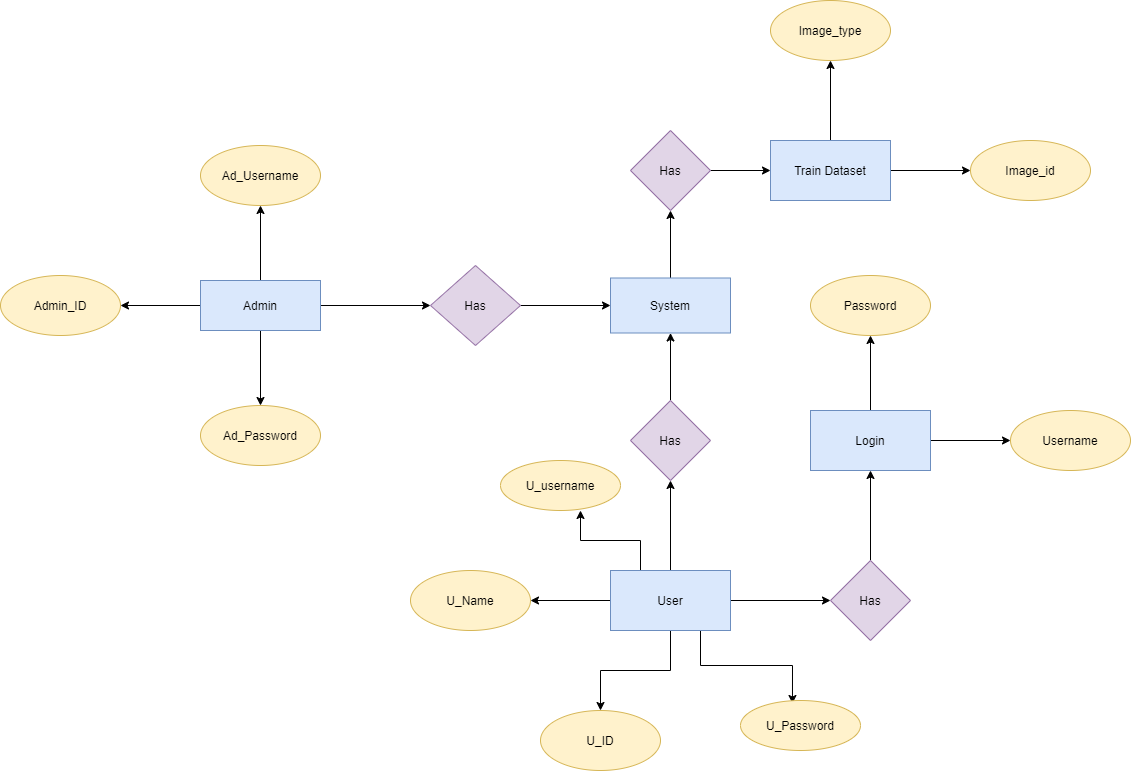
\includegraphics[width=390pt]{ER (1).png}}
	  \caption{ER Diagram}
	  \label{fig:class-dig}
	\end{figure}
\end{center} 

\section{UML DIAGRAMS} 
\item Unified Modeling Language is a standard language for writing software blueprints.The UML may be used to visualize,specify,construct and document the artifacts of a softwareintensive system.UML is process independent,although optimally it should be used in process that is use case driven,architecture-centric,iterative,and incremental.The Number of UML Diagram is available.\\

 \item Class Diagram.\\
\item Use case Diagram.\\
 \item Activity Diagram.\\
\item Sequence Diagram.\\



 \begin{center}
	\begin{figure}[!htbp]
		\centering
		\fbox{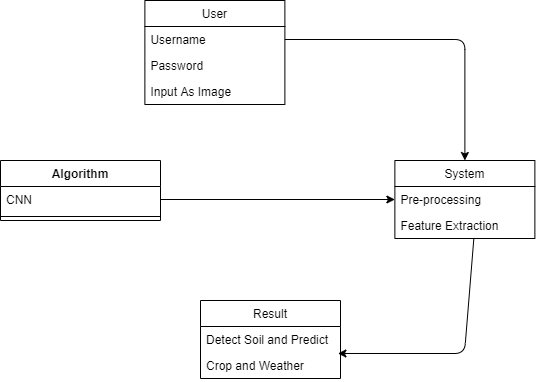
\includegraphics[width=390pt]{crop-class-Diagram.drawio.png}}
	  \caption{Class Diagram Diagram}
	  \label{fig:class-dig}
	\end{figure}
\end{center} 
\newpage
%\subsection{Use Case Diagram}

\begin{center}
	\begin{figure}[!htbp]
		\centering
		\fbox{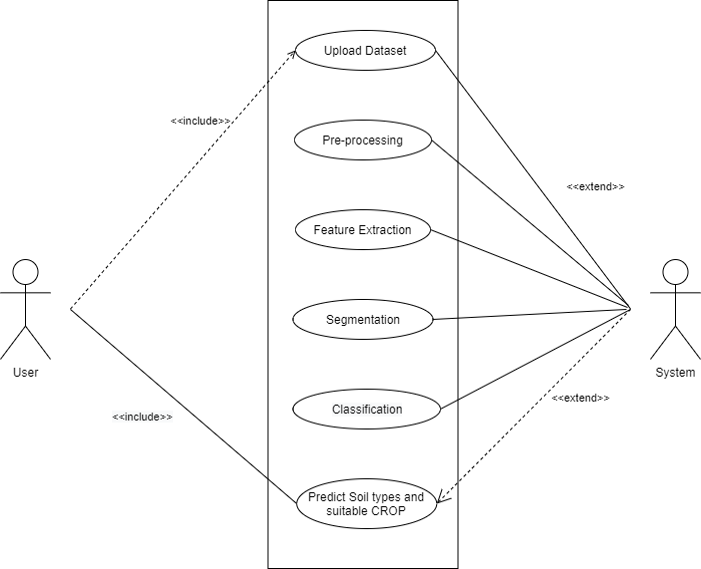
\includegraphics[width=400pt]{usecase.png}}
	  \caption{Use case Diagram}
	  \label{fig:class-dig}
	\end{figure}
\end{center} 

\newpage
%\subsection{Activity Diagram}

\begin{center}
	\begin{figure}[!htbp]
		\centering
		\fbox{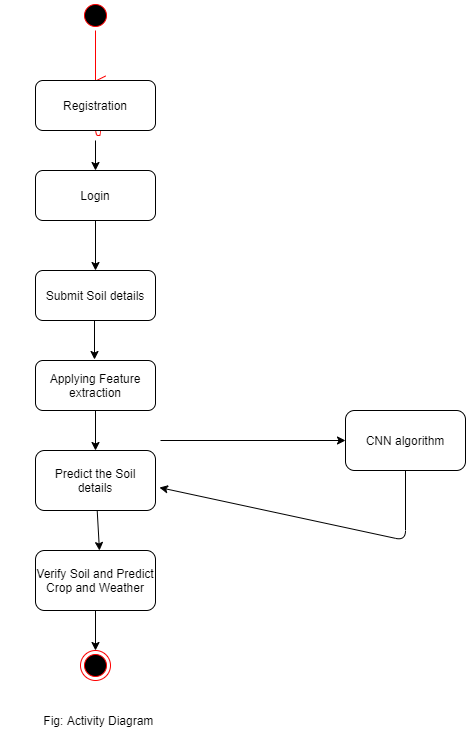
\includegraphics[width=300pt]{crop-activity-Diagram.drawio.png}}
	  \caption{Activity Diagram}
	  \label{fig:class-dig}
	\end{figure}
\end{center} 
 
\newpage
 

\newpage
 
%\subsection{Object Diagram}
 \begin{center}
	\begin{figure}[!htbp]
		\centering
		\fbox{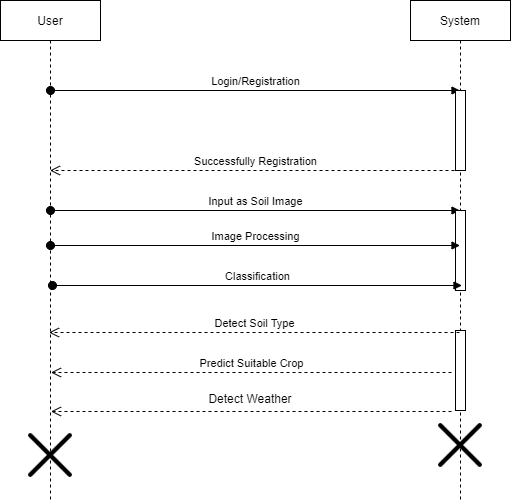
\includegraphics[width=400pt]{crop-sequence-Diagram-Page-3.drawio.png}}
	  \caption{Sequence Diagram}
	  \label{fig:class-dig}
	\end{figure}
\end{center}

\chapter{OTHER SPECIFICATION}


\section { Advantages }
\item Predicting productivity of crop in various climatic conditions can help farmer and other partners in essential basic leadership as far as agronomy and product decision. This model can be used to select the most excellent crops for the region and also its yield thereby improving the values and gain of farming also.\\
\section{Limitation}
\item Results showed that barriers to effective simulations exist because, in most instances, the input data, like climate, soil, farm management practices, and cultivar characteristics, were generally incomplete, poor in quality, and not easily accessible or usable.\\

\section{APPLICATION}
\item yield prediction is an essential task for the decision-makers at national and regional levels (e.g., the EU level) for rapid decision-making. An accurate crop yield prediction model can help farmers to decide on what to grow and when to grow. There are different approaches to crop yield prediction.

 \chapter{CONCLUSION & FUTURE SCOPE}
 \section {Conclusion}
\item 
A model is proposed for predicting soil series and providing suitable crop yield suggestion for that specific soil and weather. 
The model has been tested by applying different kinds of Deep algorithm. 
CNN shows highest accuracy in soil classification and suggests crops with less time. It gives us more accuracy as compared to existing system and gives more benefit to farmers.\\
In reference to rainfall can depict whether extra water availability is needed or not. This research work can be enhanced to higher level by availing it to whole India.
Crop diseases detection using Image Processing where users can upload picture of diseased crop and get pesticides recommendations. 
Implementation of Smart Irrigation System to monitor weather and soil conditions, plant water usage etc. to automatically alter watering schedule.


\\
\newpage
\begin{appendices}

\chapter{}

\textbf{NP-Hard NP-Complete:}\\
\vspace{1\baselineskip}\\
\textbf{What is P?}\\
\begin{itemize}
	\item P is set of all decision problems which can be solved in polynomial time by a deterministic.
	\item Since it can be solved in polynomial time, it can be verified in polynomial time.
	\item Therefore P is a subset of NP.
	
\end{itemize}

\textbf{P : } To identify road condition or road survey requires more man power, time and money. To resolve these problems we need effective system.

\begin{figure}[ht!]
	\centering
	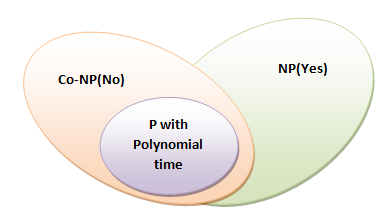
\includegraphics[width=\linewidth]{p.png}
	\caption{P Problem}
	\label{fig:P Problem}
\end{figure}

\textbf{What is NP?}\\

NP means we can solve it in polynomial time if we can break the normal rules of step-by-step computing.
\vspace{1\baselineskip}

\textbf{What is NP Hard?}\\
A problem is NP-hard if an algorithm for solving it can be translated into one for solving any NP-problem (nondeterministic polynomial time) problem. NP-hard therefore means "at least as hard as any NP-problem," although it might, in fact, be harder.\\
\vspace{1\baselineskip}

\textbf{NP-Hard:}\\
Propose system analyze the road condition and road surface. It identify bad road patches and gives notification to navigation system. For that we used inbuilt accelerometer sensor and gyroscope sensor. To improve the system result we use decision tree algorithm. Propose system has self-managing database which collect data from vehicle drivers android smart phones. This data update in real time periodically. Application utilizes this data to inform other application users about road condition.

So here in this case the ‘P’ problem is NP hard.

i.e. P=NP-Hard

\begin{figure}[ht!]
	\centering
	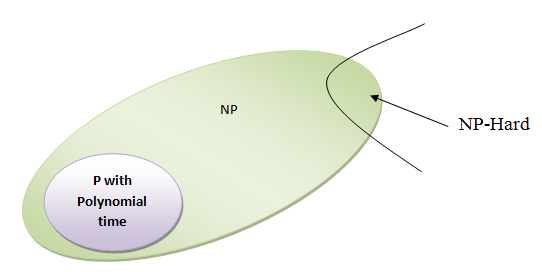
\includegraphics[width=\linewidth]{np (1).png}
	\caption{NP Problem}
	\label{fig:NP Problem}
\end{figure}

\textbf{What is NP-Complete?}\\

\begin{itemize}
	\item Since this amazing "N" computer can also do anything a normal computer can, we know that "P" problems are also in "NP".
	\item So, the easy problems are in "P" (and "NP"), but the really hard ones are *only* in "NP", and they are called "NP-complete".
	\item It is like saying there are things that People can do ("P"), there are things that Super People can do ("SP"), and there are things *only* Super People can do ("SP-complete").
\end{itemize}

\begin{figure}[ht!]
	\centering
	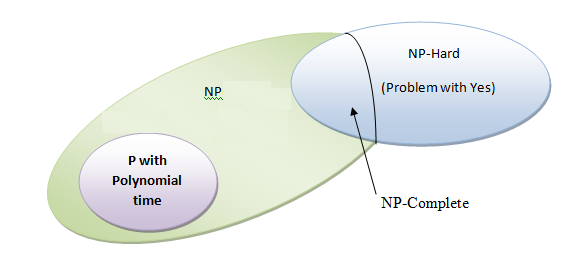
\includegraphics[width=\linewidth]{npc.png}
	\caption{NP Complete Problem}
	\label{fig:NP Complete Problem}
\end{figure}

\textbf{NP-Complete:}\\

We have used inbuilt mobile sensor to identify road conditions.

Hence the ‘P’ is NP-Complete in this case.



\chapter{}
\item 1. Sundmaeker, H.; Verdouw, C.N.; Wolfert, J.; Freire, L.P. Internet of Food and Farm 2020. In Digitising the Industry; Vermesan, O.,
Friess, P., Eds.; River Publishers: Gistrup, Denmark, 2016; pp. 129–150.
\item 2. Nguyen, G.; Dlugolinsky, S.; Bobak, M.; Tran, V.; Garcia, A.L.; Heredia, I.; Malik, P.; Hluchy, L. Machine Learning and Deep Learning
frameworks and libraries for large-scale data mining: A survey. Artif. Intell. Rev. 2019, 52, 77–124, [CrossRef]
\item 3. Hayes, M.J.; Decker, W.L. Using NOAA AVHRR data to estimate maize production in the United States Corn Belt. Int. J.
Remote Sens. 1996, 17, 3189–3200. [CrossRef]
\item 4. Bargoti, S.; Underwood, J.P. Image Segmentation for Fruit Detection and Yield Estimation in Apple Orchards. J. Field Robot. 2017,
34, 1039–1060. [CrossRef]
\item 5. Habaragamuwa, H.; Ogawa, Y.; Suzuki, T.; Shiigi, T.; Ono, M.; Kondo, N. Detecting greenhouse strawberries (mature and immature), using deep convolutional neural network. Eng. Agric. Environ. Food 2018, 11, 127–138. [CrossRef]

\end{appendices}


\newpage

{ {\bfseries \fontsize{14}{12} \selectfont \centerline{References} 
\vspace*{2\baselineskip}} \setlength{\parindent}{11mm} }
{ \setlength{\parindent}{0mm} }\\ 


\item\par [1] Arun Kumar, Naveen Kumar, Vishal Vats, “Efficient Crop Yield 
Prediction Using Machine Learning Algorithms”, International Research 
Journal of Engineering and Technology (IRJET)- e-ISSN: 2395-0056, pISSN:2395-0072, Volume: 05 Issue: 06 | June-2018
\item\par [2] Nithin Singh & saurabh chaturvedi, “Weather Forecasting Using Machine 
Learning”, 2019 International Conference on Signal Processing and 
Communication (ICSC) Volume: 05 | DEC-2019.
\item\par [3] Aakash Parmar & Mithila Sompura, "Rainfall Prediction using Machine 
Learning", 2017 International Conference on (ICIIECS) at Coimbatore 
Volume: 3 | March 2017. 
\item\par [4] Sachee Nene & Priya, R “Prediction of Crop yield using Machine 
Learning”, International Research Journal of Engineering and Technology 
(IRJET) Volume: 05 Issue: 02 | Feb-2018.
\item\par [5] Ramesh Medar & Anand M. Ambekar, “Sugarcane Crop prediction Using 
Supervised Machine Learning" published in International Journal ofIntelligent Systems and Applications Volume: 3 | August 2019. 
\item\par [6] Andrew Crane Droesch, “Machine learning methods for crop yield 
prediction and climate change impact assessment in agriculture”,
Published by IOP Publishing Ltd Volume: 05 | OCT -2018.
\item\par [7] Vinita Shah & Prachi Shah, "Groundnut Prediction Using Machine 
Learning Techniques “,published in IJSRCSEIT. UGC Journal No : 64718 
| March-2020.
\item\par [8] Renuka & Sujata Terdal, "Evaluation of Machine Learning Algorithms for 
Crop Prediction" Published in International Journal of Engineering and 
Advanced Technology (IJEAT) Volume-8 | August 2019. 
\item\par [9] P. Vinciya, Dr. A. Valarmathi, “Agriculture Analysis for Next Generation 
High Tech Farming in Data Mining” IJARCSSE,vol. 6, Issue 5, 2016
\item\par [10] Shivnath Ghosh,Santanu Koley, “Machine Learning for Soil Fertility and 
Plant Nutrient Management using Back Propagation Neural Networks” 
IJRITCC, vol. 2, Issue 2,292-297,2014. 
\\





\begin{appendices}

\end{appendices}
\end{document}
